\documentclass[12pt]{article}

\usepackage{fullpage}
\usepackage{multicol, multirow}
\usepackage{tabularx}
\usepackage{standalone}
\usepackage{listings}
\usepackage{ulem}
\usepackage{amsmath}
\usepackage{pdfpages}
\usepackage[utf8]{inputenc}
\usepackage[russian]{babel}

\newcommand{\StudentName}{Ильвохин Дмитрий}
\newcommand{\Group}{1O-106М}
\newcommand{\CourseName}{Программирование игр}
\newcommand{\LabNum}{3}
\newcommand{\Subject}{Шарики 3D}
\newcommand{\PrepName}{Аносова Н.\,П.}

\begin{document}

%\documentclass[a4paper, 12pt]{report}
\usepackage[english, russian]{babel}
\usepackage[utf8]{inputenc}
\usepackage{amssymb, amsfonts, amsmath, mathtext, cite, enumerate, float}
\usepackage{geometry}
\usepackage{chngpage}

\begin{document}

\begin{titlepage}

\newpage

\begin{center}
Московский Авиационный Институт \\*
(национальный исследовательский университет) \\*
Факультет прикладной математики и физики \\*
\hrulefill
\end{center}

\begin{center}
Кафедра вычислительной математики и программирования
\end{center}

\vspace{6em}

\begin{center}
\Large \CourseName \\
	Курсоваой проект \\
  <<\Subject>>
\end{center}

\vspace{2em}
\vspace{6em}

\begin{flushright}
	\StudentName, \\
	группа: \Group \\
\vspace{1em}
преподаватель:\\
   \PrepName \\
\end{flushright}

\vspace{\fill}

\begin{center}
Москва, 2015
\end{center}

\end{titlepage}

\end{document}
 % title page

\lstset
{
        language=Python,
        basicstyle=\footnotesize,% basic font setting
        extendedchars=\true
}

\begin{flushright}
\Large{
	\CourseName \\
	Лабораторная работа №\,\LabNum \\
	<<\Subject>> \\
	\StudentName, \Group \\
}
\end{flushright}

\subsection*{Задание}
Шарики, но уже 3D. Все тоже, что и в первой лабораторной работе, но с разницей в том,
что шарики генерируются случайным образом, их количество задается заранее в меню программы.
Параллелепипед, ограничивающий объем, в котором находятся шарики можно вращать вместе с шариками
относительно его центра, при этом вектор тяжести всегда направлен вниз.
Выбор шаров происходит по левому клику мыши, по правому клику мыши --- выбранные шары начинают движение в
сторону этого шара.
Все остальные требования (встряхивания, параметры движения и отскоков, торможение, рандомные цвета)
повторяются из первой лабораторной работы.

\subsection*{Практическая часть}
Так как в лабораторной работе требуется реализовать 3D игру, то движок LÖVE, который я использовал
для выполнения предыдущих двух лабораторных работ подходит мало. Поэтому для выполнения этой лабораторной
работы я решил использовать движок Panda3D.

Panda3D — игровой движок, включающий графику, звук, ввод-вывод, обнаружение столкновений и другие функции,
относящиеся к созданию 3D игр.

Основным языком программирования, предназначенном для работы с SDK Panda3D, является Python,
однако ядро движка написано на C++. Для обеспечения доступа к функциям ядра из Python используется
автоматическая генерация функций-обёрток.~\cite{panda_wiki}

Куб, в котором генерируются шарики построен из шести моделей квадратов, на которые наложена прозрачная
png картинка для придания эффекта прозрачности. Сами грани куба для которых рассчитываются коллизии
представляют собой шесть бесконечных плоскостей.

Для выделения шарика из камеры пускается луч и проверяется, пересекается ли этот луч с каким-то из шариков,
если да --- значит шарик подсвечивается.

Вращение куба реализовано с помощью одновременного вращения каждой грани (и плоскости ей соответствующей)
куба с помощью клавиш со стрелками.

С помощью PageUp/PageDown можно уменьшить/увеличить количество шариков в кубе.

\begin{figure}[!htb]
  \centering
    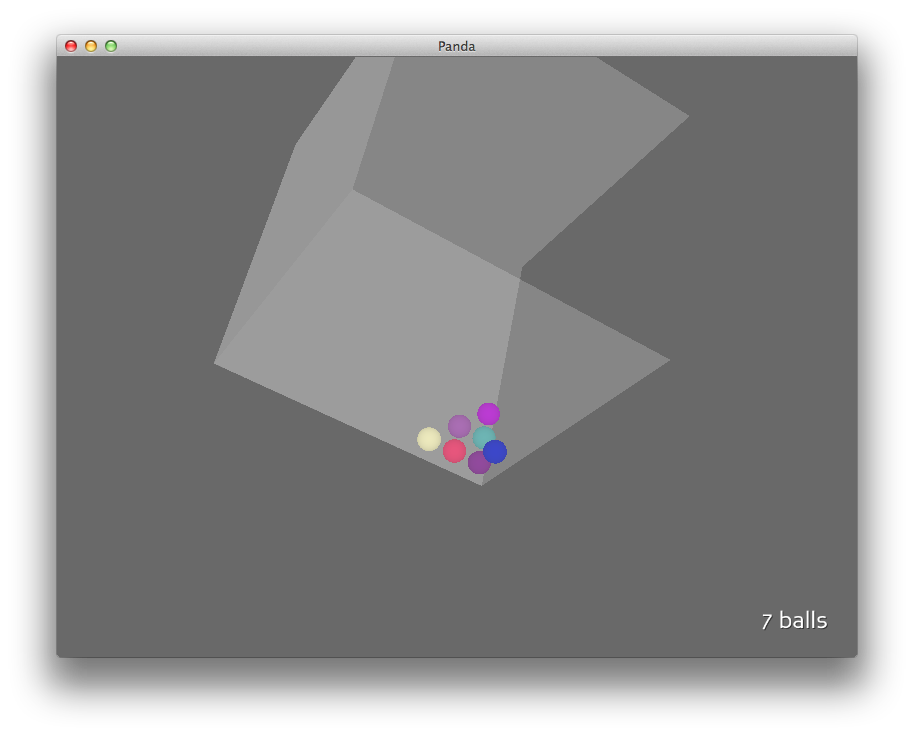
\includegraphics[scale=0.5]{pics/game.png}
   \caption{Скриншот}
    \label{fig:game}
\end{figure}

\subsection*{Выводы}
Реализовать 3D сцену оказалось сложнее, чем 2D --- пришлось вспоминать
простейшие преобразования над геометрическими объектами, которые давно
не использовал. По началу работа с новым движком шла довольно тяжело,
приходилось искать в документации нужную функцию чуть ли не для каждой строчки
кода, но потом, кажется, пошла по живее.

\begin{thebibliography}{}
\bibitem{panda_wiki} https://ru.wikipedia.org/wiki/Panda3D
\bibitem{panda} https://www.panda3d.org/
\end{thebibliography}
\end{document}

